\documentclass{article}

\usepackage[sort&compress,numbers]{natbib}
\usepackage{multicol}
\usepackage{etoolbox}
\usepackage{subfig}
\usepackage{tikz}
    \usetikzlibrary{patterns}
\usepackage{float}
\usepackage[framemethod=default]{mdframed}
\usepackage[a4paper, margin=0.75in]{geometry}
\usepackage{enumitem}
\usepackage{xcolor}

\setlist{noitemsep, topsep=0pt}

\newcommand{\TODO}[1]{\noindent{\color{red}\textbf{[TODO] #1}}}
\newcommand{\floor}[1]{\left\lfloor #1 \right\rfloor}
\newcommand{\ceil}[1]{\left\lceil #1 \right\rceil}
\newrobustcmd*{\square}[1]{\tikz{\filldraw[draw=#1,fill=#1] (0,0) rectangle (0.22cm,0.22cm);}}

\title{Improving Performance in Structured GPGPU Workloads via Specialized Thread Schedules}
\author{Narendra Prasetya}
\date{2021}

\begin{document}
\maketitle
\TODO{Maybe change title \& abstract to reflect we're mostly focussing on grouped column ordering of threads?}

\begin{abstract}
    \noindent
    High performance GPU computing has become very accessible via high level frameworks.
    These frameworks provide a limited set of operators, such as stencil, permute, fold, scan, which can manipulate data on a GPU.
    However, in most cases the compiled assembly has inefficient memory accesses with lower cache hit rates and uncoalesced accesses.
    Threads can be scheduled in such a way to minimize these inefficiencies.
    We propose several specialized thread schedules to improve performance by leveraging the structure of memory accesses in the high level GPGPU framework Accelerate.
\end{abstract}
\begin{multicols}{2}

\section{Introduction}
% Probably needs some quotes and stuff?
Modern parallel libraries, such as Accelerate, can often exploit the GPU to achieve greater parallelization and efficiency compared to traditional multithreading on CPUs.
\cite{chakravarty2011accelerating}
However these methods do not fully exploit the locality between threads with a modified scheduler.
With a smarter scheduler, programs can achieve better cache and memory utilization.
\cite{nugteren2014study}

\subsection{GPU Architecture}
Massive parallel workloads are executed on numerous cores clustered in streaming multiprocessors (SMs).
The memory is structured in a multi-level hierarchy containing a L1 cache for each SM, a shared L2 cache for all SMs and multiple banks of DRAM.
\cite{nvidia2017volta,nvidia2020ampere}

Memory can become a significant bottleneck due to the large amount of threads running concurrently.
Caches can alleviate this but is limited in size, and given a large enough problem can cause cache trashing -- the premature eviction of cache lines before any significant reuse.
\cite{dai2016model}

Data shared between threads through the cache can happen read-after-write (RAW) or read-after-read (RAR).
RAW has data dependency among tasks, for example in scan operations.
RAR has no data dependency and can be executed in any order.
\cite{tripathy2021paver}

The L1 cache in older Nvidia GPU architectures (Maxwell, Pascal) uses the least recently used (LRU) eviction policy, new architectures (Turing, Volta) uses a non-LRU eviction policy. 
\cite{jia2019dissecting, jia2018dissecting,mei2016dissecting}
\citet{jia2019dissecting} has shown that in Turing and Volta GPU's, the P-chase benchmark presented by \citet{mei2016dissecting} fails to detect the full L1 cache.
This is due to the new L1 eviction policy introduced with Volta, where cache lines can be assigned a priority.
\cite{jia2019dissecting,nvidia2021cudadocs}

A program instructs what a single thread most do, given certain runtime and constant variables.
Executing a program spawns multiple threads, each with their own thread id and corresponding block id.
These threads are grouped into cooperative thread arrays (CTA), sometimes also called a thread block.
A CTA gets executed in SIMT in groups called warps which typically contain 32 threads.
There is a maximum number of threads that can fit a CTA, so we often need multiple.

% Cache hitrate
% Memory coalescing 

\subsection{Accelerate}
Accelerate is an embedded purely functional array language in Haskell.
\cite{chakravarty2011accelerating}
Accelerate has a frontend containing the embedded language, and the backend which handles code generation and execution.
The PTX backend implements a series of CUDA skeletons.

\TODO{Explain Accelerate execution model}

\section{Related Work}

\subsection{Cache Locality}
Accessing memory on a GPU can be categorized as deterministic and non-deterministic loads.
An access is deterministic when the referenced address is generated from parameterized data such as CTA ids, thread ids, and constant parameters.
This classification can be done via backward data flow analysis. The structure of these deterministic loads can be exploited to generate better schedules for threads.
Deterministic loads are more likely to have coalesced memory access patterns. 
Non-deterministic loads will generate more memory requests due to uncoalesced memory accesses.
Koo et al. suggests that smarter CTA scheduling can improve performance.
\cite{koo2015revealing}

\subsection{CTA Clustering}
Not all applications have inter-CTA locality and intra-CTA locality can be solved within warps.
Inter-CTA locality can be categorized into:
\begin{itemize}
    \item Algorithm related locality present promising opportunities for inter-CTA reuse.
    \item Cache-line related locality result from non-aligned memory accesses or coalesced.
    \item Locality stemming from irregular data structures (pointers) often happens by accident and is thus difficult to account for.
    \item Write related applications may suffer when multiple CTAs write to the same cache line causing an eviction in the L1 cache.
    \item Streaming applications are coalesced and aligned.
\end{itemize}
\emph{Li et al.} proposes a clustering algorithm for CTAs.
For algorithmic locality, the partitioning is based on a dependency analysis on the array references.
The CTAs are then remapped according to a set of patterns.
These are executed normally or via an agent based system.
\cite{li2017locality}

\subsection{Locality Graph-Based Scheduling}
\TODO{Explain PAVER}
\cite{tripathy2021paver}

\section{Research Question}

% How much can we gain in accelerate
\begin{mdframed}
    \textbf{Research Question 1}
    \emph{What are the thread schedules for common structured GPGPU operations that result in the fastest execution?}
\end{mdframed}
A schedule optimal for one operation may not be optimal for another operation.
The optimal schedule is also dependent on the shape of the input data.
We are interested in the theoretical bounds of amounts of cache loads for a given schedule.
However, the scheduling can result in extra computation time, so we must also check with real world performance metrics.

% Comparison with current state of the art
\begin{mdframed}
    \textbf{Research Question 2}
    \emph{Is specialized structured scheduling equally or more performant than locality graph-based scheduling for structured GPGPU operations?}
\end{mdframed}
\TODO{Text}


\section{Approach}
The built-in GPU scheduler allocates threads and CTAs to streaming multiprocessors.
While the architecture does not guarantee an exact execution order of threads, it does group threads into CTAs deterministically and allocates these CTAs in a round-robin fashion.
We can therefore manipulate the scheduling by transforming the thread id.

The transformation can be implemented during the code generation phase in Accelerate, specifically by modifying the CUDA skeletons.
This allows us to manipulate the schedule depending on various (run-time) parameters such as input size, dimensionality, and GPU-architecture.

\subsection{Specialized Scheduling for Stencil Operations}
Stencil operations update an N-dimensional array according to a fixed pattern surrounding the updated element (fig. \ref{fig:stencil_access_pattern}).

\begin{figure}[H]
    \centering
    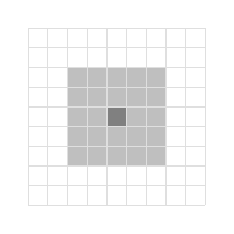
\begin{tikzpicture}[scale=0.25]
        \fill[gray!50] (2, 2) rectangle +(5, 5);
        \fill[gray!100] (4, 4) rectangle +(1, 1);
        \draw[step=1,gray!25] (0, 0) grid (9, 9);
    \end{tikzpicture}
    \caption{
        The access pattern for stencil operations on a single element \square{gray!100} that accesses \square{gray!50}.
    }
    \label{fig:stencil_access_pattern}
\end{figure}

Naive implementations of 2D stencil operations will go through the workload on a row-by-row basis.
However, if the input matrix is wide enough, data from the previous row can be unloaded before we can reuse it in the next row.
While a zigzagging pattern can help alleviate this, the issue would still persist when working on wide enough matrices.
By splitting workload into fixed width columns we can keep as much data of the previous row(s) into cache as needed.
It would add an extra initial load when threads start working on new columns, but is negligible with sufficiently long columns.

Given the stencil height $s_h$, the column width $c_w$ and the element size $e$, the required cache $M_{cache}$ is estimated with:
\[
    M_{cache} = (s_h + 1) e c_w
\]
Given the input matrix with width $I_w$ and height $I_h$, stencil width $s_w$, the amount of loads into cache $L_{cache}$ is estimated by:
\[
    L_{cache} = (c_w + s_w - 1) (I_h + s_h - 1) \ceil{\frac{I_w}{c_w}}
\]
We want to minimize $L_{cache}$ by increasing the column width. 
However, we need to keep $M_{cache}$ small enough that so everything fits on our hardware.

Earlier research suggest using tiling \cite{rivera2000tiling}, including for higher dimension stencil operations, and needs to be compared to the column method.


\TODO{Column wise access figures}
% https://virtual-graph-paper.com/NjkzZGZjNjBmMThh

\subsection{Specialized Scheduling for Matrix Multiplication}
Matrix multiplication $C = AB$ is defined as
\[
    c_{ij} = \sum^n_k{a_{ik}b_{kj}}
\]
In terms of memory accesses, for each element, a row and a column needs to be accessed (fig. \ref{fig:matmult_access_pattern}).

\begin{figure}[H]
    \centering
    \subfloat[Different arrays stacked.]{
        \centering
        \makebox[0.4\columnwidth][c]{
            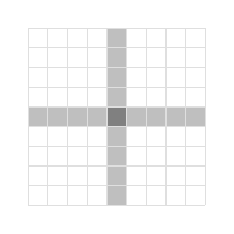
\begin{tikzpicture}[scale=0.25]
                \fill[gray!50]  (0, 4) rectangle +(9, 1);
                \fill[gray!50]  (4, 0) rectangle +(1, 9);
                \fill[gray!100] (4, 4) rectangle +(1, 1);
                \draw[step=1,gray!25] (0, 0) grid (9, 9);
            \end{tikzpicture}
        }
    }
    \qquad
    \subfloat[Different arrays separated.]{
        \centering
        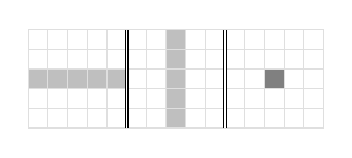
\begin{tikzpicture}[scale=0.25]
            \fill[gray!50]  (0 , 2) rectangle +(5, 1);
            \fill[gray!50]  (7 , 0) rectangle +(1, 5);
            \fill[gray!100] (12, 2) rectangle +(1, 1);
            \draw[step=1,gray!25] (0, 0) grid (15, 5);
            \draw[black, double] (5 , 0) -- +(0, 5);
            \draw[black, double] (10, 0) -- +(0, 5);
        \end{tikzpicture}
    }

    \caption{
        The access pattern for matrix multiplications on a single element \square{gray!100} that accesses \square{gray!50}.
    }
    \label{fig:matmult_access_pattern}
\end{figure}

In the ideal world, caches would be large enough to contain all the relevant matrices.
However, with inputs large enough we need to load data into cache multiple times.
By splitting the input matrices into blocks (block matrix multiplication), we can limit the amount of times a value has to be loaded into cache.

\TODO{Spatial-temporal graphs for MM}

\TODO{Column wise access for MM}

\TODO{Strassen's MM on GPUs}.
\cite{li2011strassen} % MM on GPU

\subsection{Generate and Permute}

The permutation primitive makes initializes an array with default values and then combines it with the input array according to a combination function and an index map.
From a memory point of view we are interested in the predictable memory accesses which can be defined in terms of execution parameters per thread.
These can be categorized as:
\TODO{Do I really need to differentiate local? Grouped column ordering does seem to care only about how much cache is needed and is available.}
\begin{itemize}
    \item \textbf{Localized horizontal} accesses are confined to a small horizontal area. 
    Ordering threads linearly is the optimal pattern as this preserves spatial locality.
    \item \textbf{Localized vertical} accesses are confined to a small vertical area. 
    Threads should be grouped horizontally to allow a single cache line to provide for multiple threads.

    % Furthermore, when moving to the next horizontal line of threads, the overlapping accesses should still be in cache to exploit equidistant locality\footnote{\textbf{Equidistant locality} describes both spatial and temporal locality.}.
    \item \textbf{Arbitrarily horizontal} \TODO{Description + Effect}
    \item \textbf{Arbitrarily vertical} \TODO{Description + Effect}
    \item \textbf{Singular} values are only read once and are a prime target for cache bypassing allowing other fused operations to use more cache.
    \item \textbf{Random} access are either values dependent on an earlier read value or both arbitrarily horizontal and vertical. While cache bypassing my help cache trashing when fused with another operator, it might reduce performance when accessing similar addresses.
\end{itemize}
\TODO{Propose a way to calculate column width given the accessed offsets and cache specification.}

\subsection{Fused Operations}
\TODO{Fused}
\cite{balen2020optimal}

\subsection{Scan and Fold}
Scan primitives, also known as prefix sums, have many parallel algorithms.
However, due to the RAW relationship between threads there is less freedom to tweak the scheduling.

Fold primitives are similar to scan primitives, but instead only return a single element.
The same (or partial) strategies used in scan can be used for folds.

\subsection{Planning}
\TODO{Planning}


\subsection{Preliminary Results}
To test the viability of thread scheduling, zigzagging has been implemented for stencil operations.
For a 9x9 box averaging stencil on a 4k matrix it resulted in a 13\% decrease from 20.8ms to 1.79ms in kernel run times on a RTX 2080 Super.


\end{multicols}

\bibliographystyle{unsrtnat}
\bibliography{bibliography}
\end{document}
